\section{{\color{red}Results - Scale Testing}}
\label{ResultsScaleTesting}
%
The dataset contains several zero-answers, which can happen when subjects doesn't answer on a scale. To exclude some of the zero-points that occured because of a non-answered scale two criterias is stated: 1) If all scale ratings presented on one of the pages are zero, it's probably because subjects skipped a page and 2) If there is a tendency for high ratings on a scale and a zero-answer seems unlikely, it's probably a missing answer.\\

\noindent
The different ratings on the scales in the second test are visualised on \autoref{fig:Boxplot}.
%
\begin{figure}[H]
	\centering
	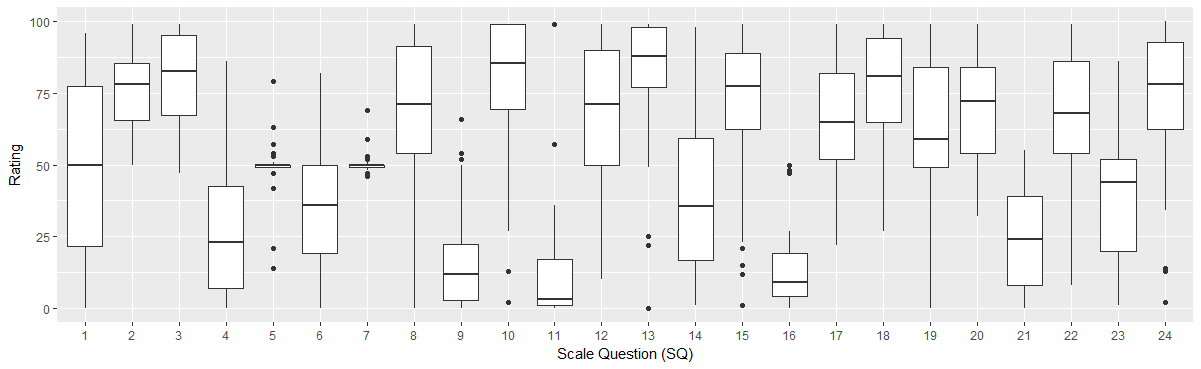
\includegraphics[width = 0.49\textwidth]{Figure/Boksplot24uden0}
	\setlength\abovecaptionskip{-1.2\baselineskip} 
	\caption{Boxplot showing the 24 variables. The boxplot contains a median, the box ranging from 25-75 \% and the whiskers from 0-25 \% and 25-100 \%, respectively.}
	\label{fig:Boxplot}
\end{figure}
\noindent
%
From the boxplots it is seen that the distribution varys. For some SQ, a big part of the scale is used (1, 4, 8, 12, 14, 19), where others a smaller part of the scale is used (2, 3, 5, 7, 9, 11, 13, 16). Furthermore some of the scale ratings looks normal distrubuted (1, 2, 6, 17, 20, 21) and others are skewed (8, 9, 10, 11, 13, 18). In some boxplot data aggregates around midpoints or terminal points (5, 7, 9, 10, 11, 13). SQ5 and SQ7 is centered around the mid point, which can reltate to the label (fine) having to wide a meaning. \\ 

\noindent
When looking at gender differences SQ4 and SQ21 seems to reveal a difference. Women rates SQ4 and SQ21 twice as high as men, which means that they experience the robot's movements more calm but also more intrusive.\\

\noindent
Conducting a PCA on the data results in the screeplot on \autoref{fig:Scree}. It shows that when using 7 dimension only 80 \% of the variance is explained, which is why PCA relating to different groups as the robot's height, distance and direction is conducted. \autoref{fig:biplot} shows the biplot relating to the robot's height. Similar biplots were made for direction and distance.
%
\begin{figure}[H]
	\centering
	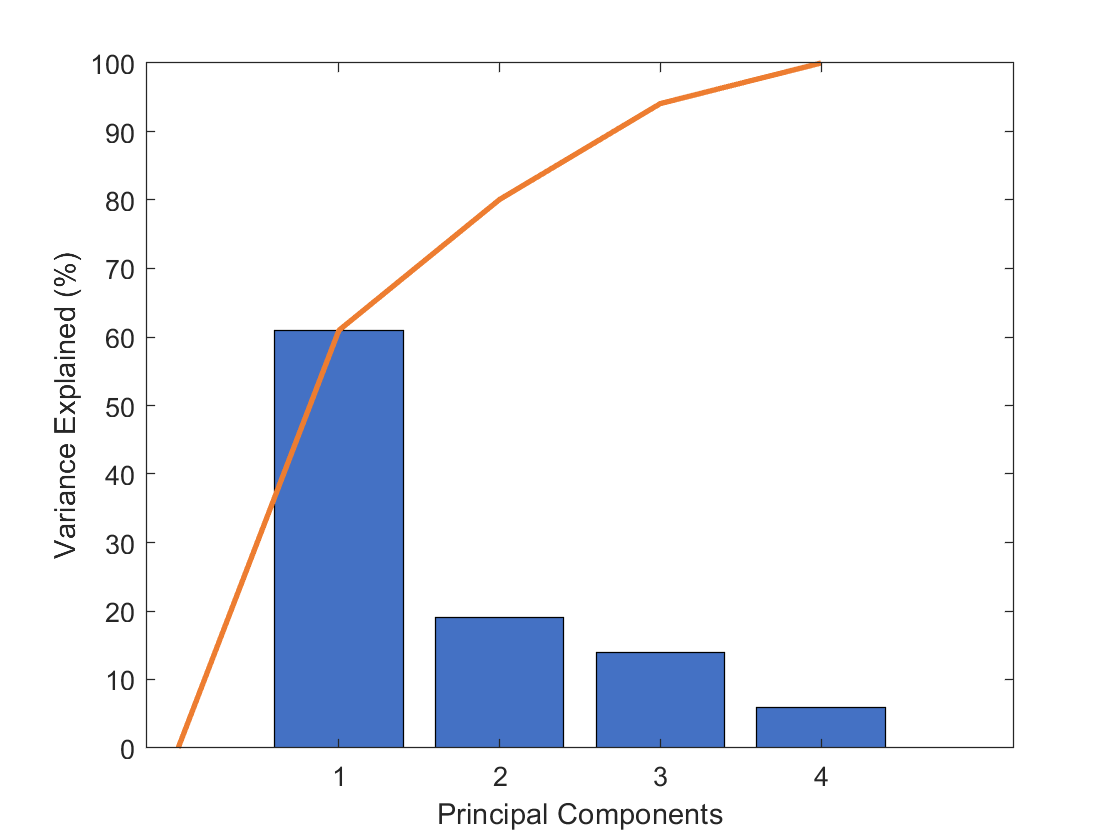
\includegraphics[width = 0.49\textwidth]{Figure/Scree.png}
	\setlength\abovecaptionskip{-1.2\baselineskip} 
	\caption{Scree plot showing the connection between the number of Principal Components and Variance Explained [\%].}
	\label{fig:Scree}
\end{figure}
\noindent
%
From \autoref{fig:biplot} it appears that SQ19 contributes the most to PC1 and SQ1 to PC2. 
%
\begin{table}[H]
	\centering
	\caption{Correlations from PCA}
	\label{tab:CorrelationsFromPCA} 
	\begin{tabular}{ c|c|c }
		\centering
		PCA & Positive correlation & Negative correlation \\ \hline
		\multirow{5}{*}{Height} & SQ8 + SQ17 & SQ2 + SQ9 \\
		& SQ10 + SQ13 & SQ4 + SQ12 \\
		& SQ12 + SQ18 & SQ12 + SQ21 \\
		& SQ14 + SQ15 & SQ16 + SQ19 \\
		&  & SQ18 + SQ21\\ \hline
		\multirow{6}{*}{Distance} & SQ1 + SQ12 & SQ2 + SQ9 \\
		& SQ7 + SQ17 & SQ5 + SQ21 \\
		& SQ8 + SQ21 & SQ10 + SQ13 \\
		& SQ10 + SQ22 & SQ13 + SQ22 \\
		&  & SQ14 + SQ16 \\	
		&  & SQ19 + SQ20 \\ \hline	
		\multirow{5}{*}{Distance} & SQ5 + SQ7 & SQ1 + SQ12 \\
		& SQ8 + SQ10 & SQ6 + SQ23 \\
		& SQ9 + SQ14 & SQ9 + SQ10 \\
		&  & SQ10 + SQ14 \\
		&  & SQ13 + SQ21 
	\end{tabular}        
\end{table}
\noindent
%
%
\begin{figure}[H]
	\centering
	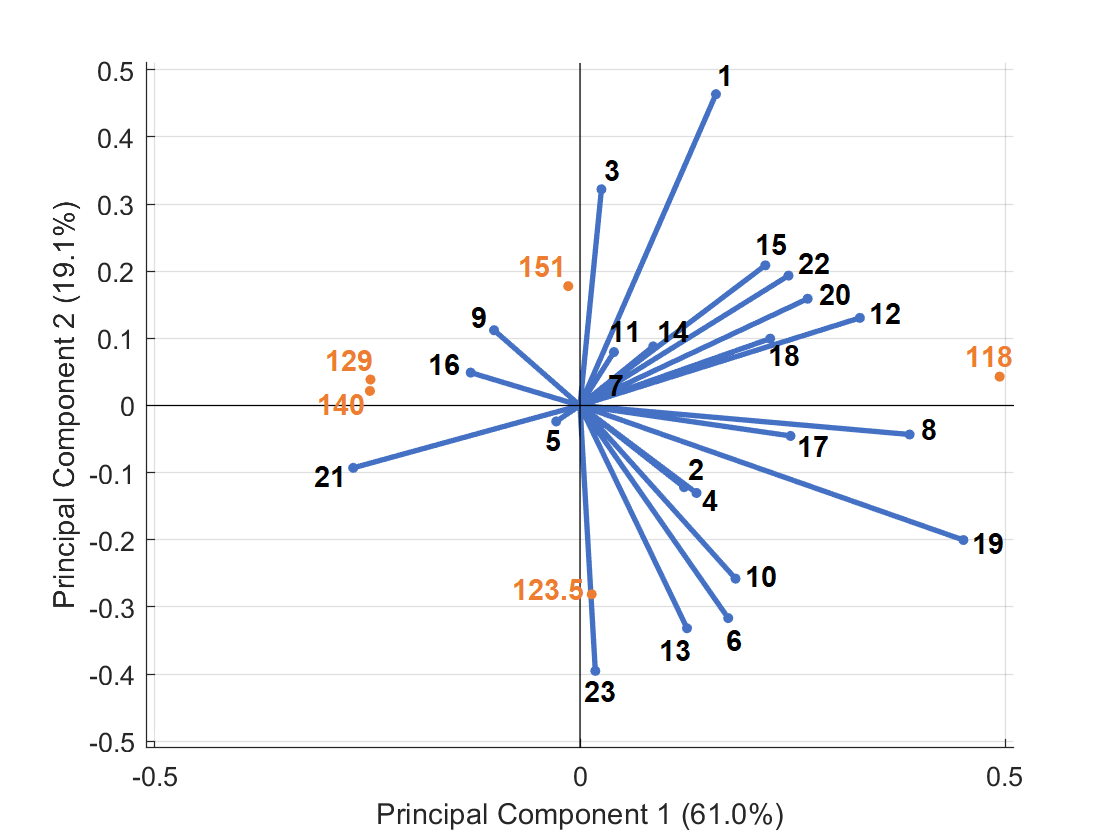
\includegraphics[width = 0.49\textwidth]{Figure/RHeight-Biplot.png}
	\setlength\abovecaptionskip{-1.2\baselineskip} 
	\caption{Biplot showing how the different variables contributes to components and which variables correlates. The black numbers denotes SQ and the red to the different heights in cm.}
	\label{fig:biplot}
\end{figure}
\noindent
%
%
\begin{figure}[H]
	\centering
	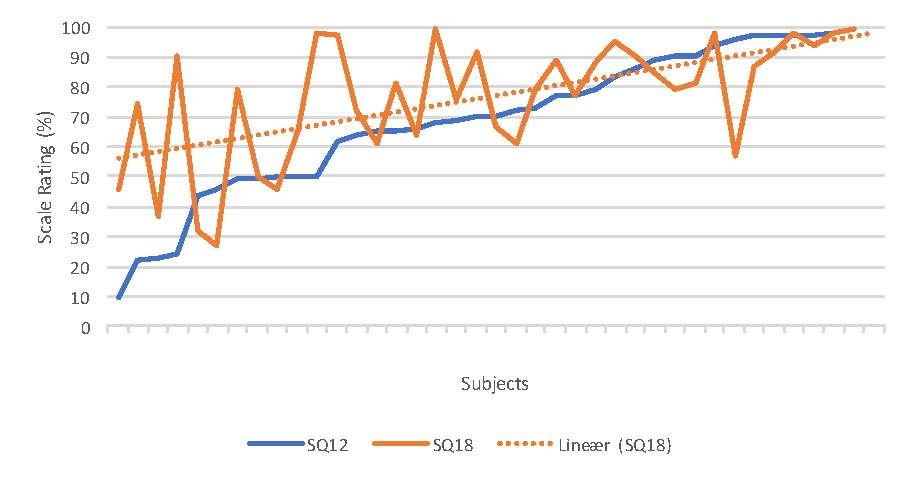
\includegraphics[width = 0.49\textwidth]{Figure/SQ12+SQ18}
	\setlength\abovecaptionskip{-1.2\baselineskip} 
	\caption{Comparison between ratings on SQ12 and SQ18 based on 41 subjects. Two were removed due to incomplete datasets.}
	\label{fig:SQ12+SQ18}
\end{figure}
\noindent
%
%
\begin{figure}[H]
	\centering
	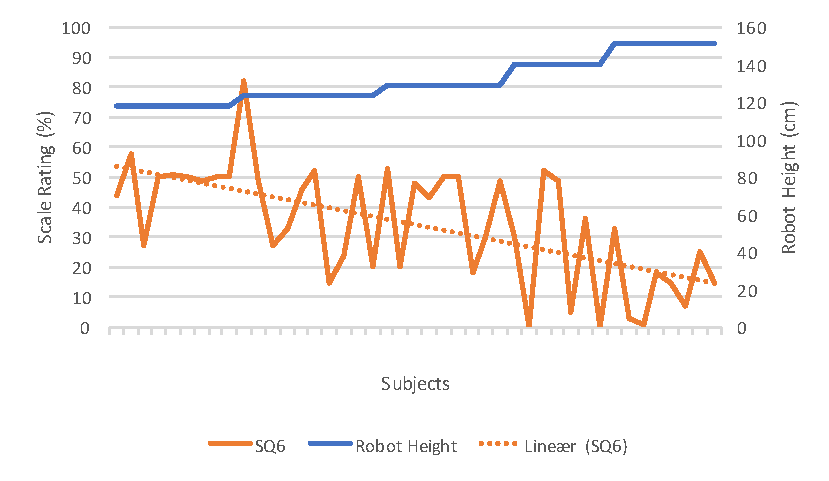
\includegraphics[width = 0.49\textwidth]{Figure/HeightSQ6}
	\setlength\abovecaptionskip{-1.2\baselineskip} 
	\caption{NEW.}
	\label{fig:HeightSQ6}
\end{figure}
\noindent
%


{\color{red} Her præsenteres resultater fra analysen af vores resultater fra anden test. Hvor resultaterne er fra Principal component analysis}
%\blankline
%
Det der tænkes at resultater skal indeholde: 
\begin{itemize}
	\item Forklare at det er eksplorativ databehandling/studie
	\item Fortælle om overordnede PCA - som ikke forklarer særlig meget af variansen.
	\item Præsenter PCA højde - hvad korrelere og er der noget der er redundant.
	\item Præsenter PCA indgangsvinkel - hvad korrelere og er der noget der er redundant.
	\item Præsenter PCA afstand - hvad korrelere og er der noget der er redundant.
\end{itemize}